%---------------
%╔═╗╔═╗╔╦╗╦ ╦╔═╗
%╚═╗║╣  ║ ║ ║╠═╝
%╚═╝╚═╝ ╩ ╚═╝╩  
%---------------


% language setup
\newcommand{\docLanguage}{ngerman}
%\newcommand{\docLanguage}{english}

% DOCUMENT SETUP
\documentclass[12pt, oneside, a4paper, \docLanguage]{report}
\usepackage[left=3cm, 
			right=2.5cm, 
			top=2.5cm, 
			bottom=2.5cm, 
			includehead, 
			includefoot]{geometry}

% line spacing
\usepackage{setspace}
\setstretch{1,25} % 15/12 --> 1.25

% encoding setup
% T1 font encoding for languages that use a latin alphabet
\usepackage[T1]{fontenc} 

% enhanced input encoding handling - utf8 for äÄüÜöÖß...
\usepackage[utf8]{inputenc}

%de­fines Adobe Times Ro­man as de­fault text font
\usepackage{mathptmx}
\usepackage{times} % needed for acronym package

%PDF linking package
\usepackage[hidelinks]{hyperref}


% Language Setup
\usepackage[\docLanguage]{babel}
% after babel - set chapter string
\AtBeginDocument{\renewcommand{\chaptername}{}}

% language specific bibliography style
\usepackage[numbers, square]{natbib}
%\setcitestyle{square,aysep={},yysep={;}}
\usepackage[fixlanguage]{babelbib}
\selectbiblanguage{\docLanguage}
% bliographystyle setup
% babel specific: babplain, babplai3, babalpha, babunsrt, bababbrv, bababbr3
\bibliographystyle{babunsrt}


% enumeration
\usepackage{enumitem}
% tabular extension tabularx
\usepackage{tabularx}

% math packages
\usepackage{amsmath}
\usepackage{nicefrac}
\usepackage{amsthm}
\usepackage{amsbsy}
\usepackage{amssymb}
\usepackage{amsfonts}
%\usepackage{MnSymbol}


%special characters
\usepackage{amssymb}
\usepackage{upgreek,textgreek}

% acronym package
\usepackage[printonlyused, footnote]{acronym}

% breakable text in \seqsplit{}
\usepackage{seqsplit}

% \textmu
\usepackage{textcomp}

% package provides a way to compile sections of a document using the same preamble as the main document
\usepackage{subfiles}

% driver-independent color extension - used by listings,tabularx
\usepackage[usenames,dvipsnames,table,xcdraw]{xcolor}

% -- SYNTAX HIGHLIGHTING --
\usepackage{listings}
%% bash command line Syntax Highlighting
\lstdefinestyle{BASH_CMD}{ 
  columns=fullflexible,            % copy pasteable listings
  language=bash,
  basicstyle=\small\sffamily,
  basicstyle   = \small \ttfamily,
  keywordstyle = [1]\small \ttfamily,
  keywordstyle = [2]\small \ttfamily,
  commentstyle = \small \ttfamily,
  numbers=none,
  captionpos=b, 
  breaklines=true,
  numberstyle=\tiny,
  numbersep=3pt,
  frame=tlrb,
  columns=fullflexible,
  backgroundcolor=\color{white!20},
  linewidth=\linewidth,
  literate=                        % replace in code
     {Ö}{{\"O}}1 
     {Ä}{{\"A}}1 
     {Ü}{{\"U}}1 
     {ß}{{\ss}}2 
     {ü}{{\"u}}1 
     {ä}{{\"a}}1 
     {ö}{{\"o}}1 
     {â}{{\^{a}}}1 
     {Â}{{\^{A}}}1 
     {ç}{{\c{c}}}1 
     {Ç}{{\c{C}}}1 
     {ğ}{{\u{g}}}1 
     {Ğ}{{\u{G}}}1 
     {ı}{{\i}}1 
     {İ}{{\.{I}}}1 
     {ş}{{\c{s}}}1 
     {Ş}{{\c{S}}}1 
}
 % adds style BASH_CMD
%% Matlab Syntax Highlighting
\colorlet{keyword}{blue!100!black!80}
\colorlet{STD}{Lavender}
\colorlet{comment}{green!90!black!90}
\definecolor{mygreen}{rgb}{0,0.6,0}
\definecolor{mygray}{rgb}{0.5,0.5,0.5}
\definecolor{mymauve}{rgb}{0.58,0,0.82}


\lstdefinestyle{BASH_SCRIPT}{ 
  language     = bash,
  basicstyle   = \footnotesize \ttfamily,
  keywordstyle = [1]\color{keyword}\bfseries,
  keywordstyle = [2]\color{STD}\bfseries,
  commentstyle = \color{mygreen}\itshape,
  backgroundcolor=\color{white},   % choose the background color; you must add \usepackage{color} 
  columns=fullflexible,            % copy pasteable listings
                                   % or \usepackage{xcolor}
  basicstyle=\footnotesize,        % the size of the fonts that are used for the code
  breakatwhitespace=false,         % sets if automatic breaks should only happen at whitespace
  breaklines=true,                 % sets automatic line breaking
  captionpos=b,                    % sets the caption-position to bottom
  extendedchars=true,              % lets you use non-ASCII characters; for 8-bits encodings only,
                                   % does not work with UTF-8
  frame=single,                    % adds a frame around the code
  keepspaces=true,                 % keeps spaces in text, useful for keeping indentation of code
                                   % (possibly needs columns=flexible)
  numbers=left,                    % where to put the line-numbers; possible values are 
                                   % (none, left, right)
  numbersep=5pt,                   % how far the line-numbers are from the code
  numberstyle=\tiny\color{mygray}, % the style that is used for the line-numbers
  rulecolor=\color{black},         % if not set, the frame-color may be changed on line-breaks
                                   % within not-black text (e.g. comments (green here))
  showspaces=false,                % show spaces everywhere adding particular underscores; it
  	                               % overrides 'showstringspaces'
  showstringspaces=false,          % underline spaces within strings only
  showtabs=false,                  % show tabs within strings adding particular underscores
  stepnumber=1,                    % the step between two line-numbers. If it's 1, each line 
                                   % will be numbered
  stringstyle=\color{mymauve},     % string literal style
  tabsize=2,                       % sets default tabsize to 2 spaces
  title=\lstname,                  % set title name
  literate=                        % replace in code
     {Ö}{{\"O}}1 
     {Ä}{{\"A}}1 
     {Ü}{{\"U}}1 
     {ß}{{\ss}}2 
     {ü}{{\"u}}1 
     {ä}{{\"a}}1 
     {ö}{{\"o}}1 
     {â}{{\^{a}}}1 
     {Â}{{\^{A}}}1 
     {ç}{{\c{c}}}1 
     {Ç}{{\c{C}}}1 
     {ğ}{{\u{g}}}1 
     {Ğ}{{\u{G}}}1 
     {ı}{{\i}}1 
     {İ}{{\.{I}}}1 
     {ş}{{\c{s}}}1 
     {Ş}{{\c{S}}}1 
} % adds style BASH_SCRIPT
% Matlab Syntax Highlighting
\colorlet{keyword}{blue!100!black!80}
\colorlet{STD}{red}
\colorlet{comment}{green!90!black!90}
\definecolor{mygreen}{rgb}{0,0.6,0}
\definecolor{mygray}{rgb}{0.5,0.5,0.5}
\definecolor{mymauve}{rgb}{0.58,0,0.82}


\lstdefinestyle{LATEX}{ 
  language     = [LaTeX]{TeX},
  basicstyle   = \footnotesize \ttfamily,
  keywordstyle = [1]\color{keyword}\bfseries,
  keywordstyle = [2]\color{comment}\bfseries,
  commentstyle = \color{mygray}\itshape,
  %backgroundcolor=\color{white},   % choose the background color; you must add \usepackage{color} 
                                   % or \usepackage{xcolor}
  basicstyle=\footnotesize,        		   % the size of the fonts that are used for the code
  breakatwhitespace=false,         % sets if automatic breaks should only happen at whitespace
  columns=fullflexible,            % copy pasteable listings
  breaklines=true,                 % sets automatic line breaking
  captionpos=c,                    % sets the caption-position to bottom
  extendedchars=true,              % lets you use non-ASCII characters; for 8-bits encodings only,
                                   % does not work with UTF-8
  frame=single,                    % adds a frame around the code
  keepspaces=true,                 % keeps spaces in text, useful for keeping indentation of code
                                   % (possibly needs columns=flexible)
  numbers=left,                    % where to put the line-numbers; possible values are 
                                   % (none, left, right)
  numbersep=4pt,                   % how far the line-numbers are from the code
  numberstyle=\tiny\color{mygray}, % the style that is used for the line-numbers
  rulecolor=\color{black},         % if not set, the frame-color may be changed on line-breaks
                                   % within not-black text (e.g. comments (green here))
  showspaces=false,                % show spaces everywhere adding particular underscores; it
  	                               % overrides 'showstringspaces'
  showstringspaces=false,          % underline spaces within strings only
  showtabs=false,                  % show tabs within strings adding particular underscores
  stepnumber=1,                    % the step between two line-numbers. If it's 1, each line 
                                   % will be numbered
  stringstyle=\color{mymauve},     % string literal style
  tabsize=2,                       % sets default tabsize to 2 spaces
  title=\lstname,                  % set title name
  literate=                        % replace in code
     {Ö}{{\"O}}1 
     {Ä}{{\"A}}1 
     {Ü}{{\"U}}1 
     {ß}{{\ss}}2 
     {ü}{{\"u}}1 
     {ä}{{\"a}}1 
     {ö}{{\"o}}1 
     {â}{{\^{a}}}1 
     {Â}{{\^{A}}}1 
     {ç}{{\c{c}}}1 
     {Ç}{{\c{C}}}1 
     {ğ}{{\u{g}}}1 
     {Ğ}{{\u{G}}}1 
     {ı}{{\i}}1 
     {İ}{{\.{I}}}1 
     {ş}{{\c{s}}}1 
     {Ş}{{\c{S}}}1 
} % adds style LATEX
%% Matlab Syntax Highlighting
\colorlet{keyword}{blue!100!black!80}
\colorlet{STD}{Lavender}
\colorlet{comment}{green!90!black!90}
\definecolor{mygreen}{rgb}{0,0.6,0}
\definecolor{mygray}{rgb}{0.5,0.5,0.5}
\definecolor{mymauve}{rgb}{0.58,0,0.82}


\lstdefinestyle{MATLAB}{ 
  language     = Matlab,
  basicstyle   = \footnotesize \ttfamily,
  keywordstyle = [1]\color{keyword}\bfseries,
  keywordstyle = [2]\color{STD}\bfseries,
  commentstyle = \color{mygreen}\itshape,
  backgroundcolor=\color{white},   % choose the background color; you must add \usepackage{color} 
                                   % or \usepackage{xcolor}
  basicstyle=\footnotesize,        % the size of the fonts that are used for the code
  breakatwhitespace=false,         % sets if automatic breaks should only happen at whitespace
  columns=fullflexible,            % copy pasteable listings
  breaklines=false,                % sets automatic line breaking
  captionpos=c,                    % sets the caption-position to bottom
  extendedchars=true,              % lets you use non-ASCII characters; for 8-bits encodings only,
                                   % does not work with UTF-8
  frame=single,                    % adds a frame around the code
  keepspaces=true,                 % keeps spaces in text, useful for keeping indentation of code
                                   % (possibly needs columns=flexible)
  numbers=left,                    % where to put the line-numbers; possible values are 
                                   % (none, left, right)
  numbersep=5pt,                   % how far the line-numbers are from the code
  numberstyle=\tiny\color{mygray}, % the style that is used for the line-numbers
  rulecolor=\color{black},         % if not set, the frame-color may be changed on line-breaks
                                   % within not-black text (e.g. comments (green here))
  showspaces=false,                % show spaces everywhere adding particular underscores; it
  	                               % overrides 'showstringspaces'
  showstringspaces=false,          % underline spaces within strings only
  showtabs=false,                  % show tabs within strings adding particular underscores
  stepnumber=1,                    % the step between two line-numbers. If it's 1, each line 
                                   % will be numbered
  stringstyle=\color{mymauve},     % string literal style
  tabsize=2,                       % sets default tabsize to 2 spaces
  title=\lstname,                  % set title name
  literate=                        % replace in code
     {Ö}{{\"O}}1 
     {Ä}{{\"A}}1 
     {Ü}{{\"U}}1 
     {ß}{{\ss}}2 
     {ü}{{\"u}}1 
     {ä}{{\"a}}1 
     {ö}{{\"o}}1 
     {â}{{\^{a}}}1 
     {Â}{{\^{A}}}1 
     {ç}{{\c{c}}}1 
     {Ç}{{\c{C}}}1 
     {ğ}{{\u{g}}}1 
     {Ğ}{{\u{G}}}1 
     {ı}{{\i}}1 
     {İ}{{\.{I}}}1 
     {ş}{{\c{s}}}1 
     {Ş}{{\c{S}}}1 
} % adds style MATLAB
% Matlab Syntax Highlighting
\colorlet{keyword}{blue!100!black!80}
\colorlet{STD}{Lavender}
\colorlet{comment}{green!90!black!90}
\definecolor{mygreen}{rgb}{0,0.6,0}
\definecolor{mygray}{rgb}{0.5,0.5,0.5}
\definecolor{mymauve}{rgb}{0.58,0,0.82}


\lstdefinestyle{PYTHON}{ 
  language     = Python,
  basicstyle   = \footnotesize \ttfamily,
  keywordstyle = [1]\color{keyword}\bfseries,
  keywordstyle = [2]\color{STD}\bfseries,
  commentstyle = \color{mygreen}\itshape,
  backgroundcolor=\color{white},   % choose the background color; you must add \usepackage{color} 
                                   % or \usepackage{xcolor}
  basicstyle=\footnotesize,        % the size of the fonts that are used for the code
  columns=fullflexible,            % copy pasteable listings
  breakatwhitespace=false,         % sets if automatic breaks should only happen at whitespace
  breaklines=false,                % sets automatic line breaking
  captionpos=c,                    % sets the caption-position to bottom
  extendedchars=true,              % lets you use non-ASCII characters; for 8-bits encodings only,
                                   % does not work with UTF-8
  frame=single,                    % adds a frame around the code
  keepspaces=true,                 % keeps spaces in text, useful for keeping indentation of code
                                   % (possibly needs columns=flexible)
  numbers=left,                    % where to put the line-numbers; possible values are 
                                   % (none, left, right)
  numbersep=5pt,                   % how far the line-numbers are from the code
  numberstyle=\tiny\color{mygray}, % the style that is used for the line-numbers
  rulecolor=\color{black},         % if not set, the frame-color may be changed on line-breaks
                                   % within not-black text (e.g. comments (green here))
  showspaces=false,                % show spaces everywhere adding particular underscores; it
  	                               % overrides 'showstringspaces'
  showstringspaces=false,          % underline spaces within strings only
  showtabs=false,                  % show tabs within strings adding particular underscores
  stepnumber=1,                    % the step between two line-numbers. If it's 1, each line 
                                   % will be numbered
  stringstyle=\color{mymauve},     % string literal style
  tabsize=2,                       % sets default tabsize to 2 spaces
  title=\lstname,                  % set title name
  literate=                        % replace in code
     {Ö}{{\"O}}1 
     {Ä}{{\"A}}1 
     {Ü}{{\"U}}1 
     {ß}{{\ss}}2 
     {ü}{{\"u}}1 
     {ä}{{\"a}}1 
     {ö}{{\"o}}1 
     {â}{{\^{a}}}1 
     {Â}{{\^{A}}}1 
     {ç}{{\c{c}}}1 
     {Ç}{{\c{C}}}1 
     {ğ}{{\u{g}}}1 
     {Ğ}{{\u{G}}}1 
     {ı}{{\i}}1 
     {İ}{{\.{I}}}1 
     {ş}{{\c{s}}}1 
     {Ş}{{\c{S}}}1 
} % adds style PYTHON
%% Matlab Syntax Highlighting
\colorlet{keyword}{blue!100!black!80}
\colorlet{STD}{Lavender}
\colorlet{comment}{green!90!black!90}
\definecolor{mygreen}{rgb}{0,0.6,0}
\definecolor{mygray}{rgb}{0.5,0.5,0.5}
\definecolor{mymauve}{rgb}{0.58,0,0.82}


\lstdefinestyle{CPP}{ 
  language     = C++,
  basicstyle   = \footnotesize \ttfamily,
  keywordstyle = [1]\color{keyword}\bfseries,
  keywordstyle = [2]\color{STD}\bfseries,
  commentstyle = \color{mygreen}\itshape,
  backgroundcolor=\color{white},   % choose the background color; you must add \usepackage{color} 
                                   % or \usepackage{xcolor}
  columns=fullflexible,            % copy pasteable listings
  basicstyle=\footnotesize,        % the size of the fonts that are used for the code
  breakatwhitespace=false,         % sets if automatic breaks should only happen at whitespace
  breaklines=false,                % sets automatic line breaking
  captionpos=c,                    % sets the caption-position to bottom
  extendedchars=true,              % lets you use non-ASCII characters; for 8-bits encodings only,
                                   % does not work with UTF-8
  frame=single,                    % adds a frame around the code
  keepspaces=true,                 % keeps spaces in text, useful for keeping indentation of code
                                   % (possibly needs columns=flexible)
  numbers=left,                    % where to put the line-numbers; possible values are 
                                   % (none, left, right)
  numbersep=5pt,                   % how far the line-numbers are from the code
  numberstyle=\tiny\color{mygray}, % the style that is used for the line-numbers
  rulecolor=\color{black},         % if not set, the frame-color may be changed on line-breaks
                                   % within not-black text (e.g. comments (green here))
  showspaces=false,                % show spaces everywhere adding particular underscores; it
  	                               % overrides 'showstringspaces'
  showstringspaces=false,          % underline spaces within strings only
  showtabs=false,                  % show tabs within strings adding particular underscores
  stepnumber=1,                    % the step between two line-numbers. If it's 1, each line 
                                   % will be numbered
  stringstyle=\color{mymauve},     % string literal style
  tabsize=2,                       % sets default tabsize to 2 spaces
  title=\lstname,                  % set title name
  literate=                        % replace in code
     {Ö}{{\"O}}1 
     {Ä}{{\"A}}1 
     {Ü}{{\"U}}1 
     {ß}{{\ss}}2 
     {ü}{{\"u}}1 
     {ä}{{\"a}}1 
     {ö}{{\"o}}1 
     {â}{{\^{a}}}1 
     {Â}{{\^{A}}}1 
     {ç}{{\c{c}}}1 
     {Ç}{{\c{C}}}1 
     {ğ}{{\u{g}}}1 
     {Ğ}{{\u{G}}}1 
     {ı}{{\i}}1 
     {İ}{{\.{I}}}1 
     {ş}{{\c{s}}}1 
     {Ş}{{\c{S}}}1 
} % adds style CPP
%% Matlab Syntax Highlighting
\colorlet{keyword}{blue!100!black!80}
\colorlet{STD}{Lavender}
\colorlet{comment}{green!90!black!90}
\definecolor{mygreen}{rgb}{0,0.6,0}
\definecolor{mygray}{rgb}{0.5,0.5,0.5}
\definecolor{mymauve}{rgb}{0.58,0,0.82}


\lstdefinestyle{C}{ 
  language     = C,
  basicstyle   = \footnotesize \ttfamily,
  keywordstyle = [1]\color{keyword}\bfseries,
  keywordstyle = [2]\color{STD}\bfseries,
  commentstyle = \color{mygreen}\itshape,
  backgroundcolor=\color{white},   % choose the background color; you must add \usepackage{color} 
  columns=fullflexible,            % copy pasteable listings
                                   % or \usepackage{xcolor}
  basicstyle=\footnotesize,        % the size of the fonts that are used for the code
  breakatwhitespace=false,         % sets if automatic breaks should only happen at whitespace
  breaklines=false,                % sets automatic line breaking
  captionpos=c,                    % sets the caption-position to bottom
  extendedchars=true,              % lets you use non-ASCII characters; for 8-bits encodings only,
                                   % does not work with UTF-8
  frame=single,                    % adds a frame around the code
  keepspaces=true,                 % keeps spaces in text, useful for keeping indentation of code
                                   % (possibly needs columns=flexible)
  numbers=left,                    % where to put the line-numbers; possible values are 
                                   % (none, left, right)
  numbersep=5pt,                   % how far the line-numbers are from the code
  numberstyle=\tiny\color{mygray}, % the style that is used for the line-numbers
  rulecolor=\color{black},         % if not set, the frame-color may be changed on line-breaks
                                   % within not-black text (e.g. comments (green here))
  showspaces=false,                % show spaces everywhere adding particular underscores; it
  	                               % overrides 'showstringspaces'
  showstringspaces=false,          % underline spaces within strings only
  showtabs=false,                  % show tabs within strings adding particular underscores
  stepnumber=1,                    % the step between two line-numbers. If it's 1, each line 
                                   % will be numbered
  stringstyle=\color{mymauve},     % string literal style
  tabsize=2,                       % sets default tabsize to 2 spaces
  title=\lstname,                  % set title name
  literate=                        % replace in code
     {Ö}{{\"O}}1 
     {Ä}{{\"A}}1 
     {Ü}{{\"U}}1 
     {ß}{{\ss}}2 
     {ü}{{\"u}}1 
     {ä}{{\"a}}1 
     {ö}{{\"o}}1 
     {â}{{\^{a}}}1 
     {Â}{{\^{A}}}1 
     {ç}{{\c{c}}}1 
     {Ç}{{\c{C}}}1 
     {ğ}{{\u{g}}}1 
     {Ğ}{{\u{G}}}1 
     {ı}{{\i}}1 
     {İ}{{\.{I}}}1 
     {ş}{{\c{s}}}1 
     {Ş}{{\c{S}}}1 
} % adds style C
%% JSON Syntax Highlighting
\colorlet{keyword}{blue!100!black!80}
\colorlet{STD}{Lavender}
\colorlet{comment}{green!90!black!90}
\definecolor{mygreen}{rgb}{0,0.6,0}
\definecolor{mygray}{rgb}{0.5,0.5,0.5}
\definecolor{mymauve}{rgb}{0.58,0,0.82}

\newcommand\JSONnumbervaluestyle{\color{blue}}
\newcommand\JSONstringvaluestyle{\color{red}}

\newif\ifcolonfoundonthisline

\makeatletter

\lstdefinelanguage{json}
{
  showstringspaces    = false,
  keywords            = {false,true},
  alsoletter          = 0123456789.,
  morestring          = [s]{"}{"},
  morestring          = [s]{'}{'},
  stringstyle         = \ifcolonfoundonthisline\JSONstringvaluestyle\fi,
  MoreSelectCharTable =%
    \lst@DefSaveDef{`:}\colon@json{\processColon@json},
  basicstyle          = \ttfamily,
  keywordstyle        = \ttfamily\bfseries,
}

% flip the switch if a colon is found in Pmode
\newcommand\processColon@json{
  \colon@json%
  \ifnum\lst@mode=\lst@Pmode%
    \global\colonfoundonthislinetrue%
  \fi
}

\lst@AddToHook{Output}{%
  \ifcolonfoundonthisline%
    \ifnum\lst@mode=\lst@Pmode%
      \def\lst@thestyle{\JSONnumbervaluestyle}%
    \fi
  \fi
  %override by keyword style if a keyword is detected!
  \lsthk@DetectKeywords% 
}

% reset the switch at the end of line
\lst@AddToHook{EOL}%
  {\global\colonfoundonthislinefalse}

\makeatother



\lstdefinestyle{JSON}{ 
  language     = json,
  basicstyle   = \footnotesize \ttfamily,
  keywordstyle = [1]\color{keyword}\bfseries,
  keywordstyle = [2]\color{STD}\bfseries,
  commentstyle = \color{mygreen}\itshape,
  backgroundcolor=\color{white},   % choose the background color; you must add \usepackage{color} 
                                   % or \usepackage{xcolor}
  basicstyle=\footnotesize,        % the size of the fonts that are used for the code
  columns=fullflexible,            % copy pasteable listings
  breakatwhitespace=false,         % sets if automatic breaks should only happen at whitespace
  breaklines=false,                % sets automatic line breaking
  captionpos=c,                    % sets the caption-position to bottom
  extendedchars=true,              % lets you use non-ASCII characters; for 8-bits encodings only,
                                   % does not work with UTF-8
  frame=single,                    % adds a frame around the code
  keepspaces=true,                 % keeps spaces in text, useful for keeping indentation of code
                                   % (possibly needs columns=flexible)
  numbers=left,                    % where to put the line-numbers; possible values are 
                                   % (none, left, right)
  numbersep=5pt,                   % how far the line-numbers are from the code
  numberstyle=\tiny\color{mygray}, % the style that is used for the line-numbers
  rulecolor=\color{black},         % if not set, the frame-color may be changed on line-breaks
                                   % within not-black text (e.g. comments (green here))
  showspaces=false,                % show spaces everywhere adding particular underscores; it
  	                               % overrides 'showstringspaces'
  showstringspaces=false,          % underline spaces within strings only
  showtabs=false,                  % show tabs within strings adding particular underscores
  stepnumber=1,                    % the step between two line-numbers. If it's 1, each line 
                                   % will be numbered
  stringstyle=\color{mymauve},     % string literal style
  tabsize=2,                       % sets default tabsize to 2 spaces
  title=\lstname,                  % set title name
  literate=                        % replace in code
     {Ö}{{\"O}}1 
     {Ä}{{\"A}}1 
     {Ü}{{\"U}}1 
     {ß}{{\ss}}2 
     {ü}{{\"u}}1 
     {ä}{{\"a}}1 
     {ö}{{\"o}}1 
     {â}{{\^{a}}}1 
     {Â}{{\^{A}}}1 
     {ç}{{\c{c}}}1 
     {Ç}{{\c{C}}}1 
     {ğ}{{\u{g}}}1 
     {Ğ}{{\u{G}}}1 
     {ı}{{\i}}1 
     {İ}{{\.{I}}}1 
     {ş}{{\c{s}}}1 
     {Ş}{{\c{S}}}1 
} % adds style JSON

% HEADLINE CFG
\usepackage{fancyhdr} % Headers and footers
\usepackage{lastpage}
\usepackage{ifthen}
\setlength{\headheight}{1.5cm}
%\pagestyle{fancy} % All pages have headers and footers
% override plain page style for \part, \chapter or 
% \maketitle, which implicit specifies plain page style
\fancypagestyle{plain} 
{
	\fancyhead[L]{}
	\fancyhead[C]{}
	\fancyhead[R]{}
	\fancyfoot[L]{}
	\fancyfoot[C]{\thepage}
	\fancyfoot[R]{}
}
% set list pagestyle
\fancypagestyle{preface} 
{
	\fancyhead[L]{}
	\fancyhead[C]{}
	\fancyhead[R]{}
	\fancyfoot[L]{}
	\fancyfoot[C]{\thepage}
	\fancyfoot[R]{}
}
% set default pagestyle
\fancypagestyle{default} 
{
	\fancyhead{} % Blank out the default header
	\fancyfoot{} % Blank out the default footer
	\fancyhead[L]{}
	\fancyhead[C]{}
	\fancyhead[R]{}
	\fancyfoot[L]{}
	\fancyfoot[C]{\thepage}
	\fancyfoot[R]{}
}
%\fancypagestyle{default} 
{
\fancyhead[L]{\ifthenelse{\isodd{\value{page}}}{\arabic{chapter} \rightmark}{}}
\fancyhead[R]{\thepage}
}

\renewcommand{\chaptermark}[1]{\markright{#1}{}}
\renewcommand{\sectionmark}[1]{\markright{#1}{}}
\renewcommand{\headrulewidth}{0pt}
\renewcommand{\footrulewidth}{0pt}

% PICTURE CFG 
\usepackage{verbatim}
\usepackage{graphicx}
\usepackage{epstopdf}
\usepackage{caption}
\usepackage[list=true,listformat=simple]{subcaption}
% floating prevention packages
\usepackage{float}    % used with [H] positioning parameter
\usepackage{placeins} % \FloatBarrier 
% tikz packages
\usepackage{tikz}
\usepackage{standalone}
\usepackage{pgfplots}

% include only specified tex files - uncommend here
\includeonly{preface/cover,
             preface/abstract,
             preface/tableofcontents,
             preface/listoffigures,
             preface/listoftables,
             preface/lstlistoflistings,
             appendix/bibliography}

%-------------------
%╔═╗╔╦╗╦═╗╦╔╗╔╔═╗╔═╗
%╚═╗ ║ ╠╦╝║║║║║ ╦╚═╗
%╚═╝ ╩ ╩╚═╩╝╚╝╚═╝╚═╝
%-------------------
\newcommand{\strLecture}{Signale, Systeme und Sensoren}
\newcommand{\strDate}{\today}
\newcommand{\strAuthorA}{M. Rudolph}
\newcommand{\strAuthorB}{B. Jasper}
\newcommand{\strAuthorC}{T. Schoch}
\newcommand{\strAuthorAEmail}{marvin.rudolph@htwg-konstanz.de}
\newcommand{\strAuthorBEmail}{benjamin.jasper@htwg-konstanz.de}
\newcommand{\strAuthorCEmail}{tobias.schoch@htwg-konstanz.de}
% Versuchsbeschreibung 
\newcommand{\strTopic}{Digitalisierung}
\newcommand{\strAbstract}{
In diesem Versuch wird die Umwandlung von analogen in digitale Daten und umgekehrt untersucht.
Dabei wollen wir vorallem auf folgende Themen eingehen:
\newline
\newline
Der Umgang mit Analog-zu-Digital und Digital-zu-Analog Wandlern, die Messungen der Genauigkeit der AD- und DA- Wandlung, die Untersuchung des Zeitverhaltens der DA-Wandlung und die praktische Erfahrung mit dem Abtasttheorem.
\newline
Diese Themen behandeln wir mit der Multifunktionsbox ME-RedLab USB-1208LS. Mit dieser wandeln wir Analoge- in die Digitale Signale und umgekehrt.
\newline
So werden wir Werte auslesen aus der Mulitfunktionsbox und Werte auf die Multifunktionsbox geben.
Zudem werden wir Genauigkeit der AD-Wandlung testen, sowie die Genauigkeit der DA-Wandlung.
\newline
Im Anschluss werden wir das Zeitverhalten der DA-Wandlung überprüfen und das Abtasttheorem behandeln.}
% hyperref customization
\hypersetup{
	pdftitle     = {\strTopic}, % title
	pdfsubject   = {\strLecture}, % subject of the document
	pdfauthor    = {\strAuthorA, \strAuthorB, \strAuthorC}, % author
	pdfkeywords  = {}, % list of keywords
	pdfcreator   = {}, % creator of the document
	pdfproducer  = {}, % producer of the document
	colorlinks   = false, % false: boxed links; true: colored links
	linkcolor    = red, % color of internal links (change box color with linkbordercolor)
    citecolor    = green, % color of links to bibliography
    filecolor    = magenta, % color of file links
    urlcolor     = cyan, % color of external links
	%bookmarks    = true, % show bookmarks bar?
	unicode	     = true, % non-Latin characters in Acrobat’s bookmarks
	pdftoolbar   = true, % show Acrobat’s toolbar?
	pdfmenubar   = true, % show Acrobat’s menu?
    pdffitwindow = false, % window fit to page when opened
	pdfnewwindow = true % links in new PDF window
}

%-----------------------------------------
% ╔╗ ╔═╗╔═╗╦╔╗╔  ╔╦╗╔═╗╔═╗╦ ╦╔╦╗╔═╗╔╗╔╔╦╗ 
% ╠╩╗║╣ ║ ╦║║║║   ║║║ ║║  ║ ║║║║║╣ ║║║ ║  
% ╚═╝╚═╝╚═╝╩╝╚╝  ═╩╝╚═╝╚═╝╚═╝╩ ╩╚═╝╝╚╝ ╩  
%-----------------------------------------
\setcounter{chapter}{-1}
\begin{document}
\pagenumbering{Roman} 

\setcounter{section}{0}

\begin{titlepage}

\vspace*{-3.5cm}

\begin{flushleft}
\hspace*{-1cm} 
\includegraphics[width=15.7cm]{preface/htwg-logo.png}
\end{flushleft}

\vspace{1cm}

\begin{center}
	\large{
		\textbf{\strLecture} \\[2cm]
	}
	\Huge{
		\textbf{\strTopic} \\[2cm]
	}
	\Large{
		%\textbf{\strAuthorA, \strAuthorB}} \\[3cm]
		\textbf{\strAuthorA, \strAuthorB, \strAuthorC}} \\[3cm]
	\large{
		\textbf{} \\[2.3cm]
	}
	
	\large{
		\textbf{Konstanz, \strDate}
	}
\end{center}

\end{titlepage}
\thispagestyle{empty}



\begin{center}
{\Large \textbf{Zusammenfassung (Abstract)}}
\end{center}

\bigskip

\begin{center}
	\begin{tabular}{p{2.8cm}p{5cm}p{5cm}}
		Thema: & \multicolumn{2}{p{10cm}}{\raggedright\strTopic} \\
		 & & \\
		Autoren: & \strAuthorA & \href{mailto:\strAuthorAEmail}{\strAuthorAEmail} \\
		 & \strAuthorB & \href{mailto:\strAuthorBEmail}{\strAuthorBEmail} \\
%		 & \strAuthorC & \href{mailto:\strAuthorCEmail}{\strAuthorCEmail} \\
		 & & \\
		Betreuer: & Prof. Dr. Matthias O. Franz & \href{mailto:mfranz@htwg-konstanz.de}{mfranz@htwg-konstanz.de} \\
		 &  Jürgen Keppler & \href{mailto:juergen.keppler@htwg-konstanz.de}{juergen.keppler@htwg-konstanz.de} \\
		 &  Christoph Kaiser & \href{mailto:Christop.kaiser@htwg-konstanz.de}{ch241kai@htwg-konstanz.de} \\
	\end{tabular}
\end{center}

\bigskip

\noindent
\strAbstract

\thispagestyle{preface}



\clearpage

%
% TABLE OF CONTENTS
%
\pagestyle{preface}
%
% TABLE OF CONTENTS
%
\tableofcontents
\newpage


%
% Abbildungsverzeichnis
%
%
% Abbildungsverzeichnis
%
\phantomsection
\addcontentsline{toc}{chapter}{Abbildungsverzeichnis}
\listoffigures
\thispagestyle{preface}
\newpage
\clearpage

%
% Tabellenverzeichnis
%
%
% Tabellenverzeichnis
%
\phantomsection
\addcontentsline{toc}{chapter}{Tabellenverzeichnis}
\listoftables
\thispagestyle{preface}
\newpage
\clearpage

%
% Listingverzeichnis
%
%
% Listingverzeichnis
%
\phantomsection
\renewcommand\lstlistingname{Listing}
\renewcommand\lstlistlistingname{Listingverzeichnis}
\lstlistoflistings
\addcontentsline{toc}{chapter}{Listingverzeichnis}
\thispagestyle{preface}
\newpage
\clearpage


%--------------------------
% ╔═╗╦ ╦╔═╗╔═╗╔╦╗╔═╗╦═╗╔═╗ 
% ║  ╠═╣╠═╣╠═╝ ║ ║╣ ╠╦╝╚═╗ 
% ╚═╝╩ ╩╩ ╩╩   ╩ ╚═╝╩╚═╚═╝ 
%--------------------------

\pagenumbering{arabic} 
\setcounter{page}{1} 
\pagestyle{default}

%
% CHAPTER Einleitung
%
\chapter{Einleitung}
\label{chap:EINL}
In diesem Versuch wird die Umwandlung von analogen in digitale Daten und umgekehrt untersucht.
Die Lernziele in dem letzten Versuch der Versuchsreihe sind unter anderem:
\begin{itemize}
\item Umgang mit Analog-zu-Digital und Digital-zu-Analog Wandlern
\item Messung der Genauigkeit der AD- und DA- Wandlung
\item Untersuchung des Zeitverhaltens der DA-Wandlung
\item Praktische Erfahrung mit dem Abtasttheorem
\newline
\end{itemize}
Diese Themen behandeln wir mit der Multifunktionsbox ME-RedLab USB-1208LS. Mit dieser wandeln wir Analoge- in die Digitale Signale und umgekehrt.
\newline
So werden wir Werte auslesen aus der Mulitfunktionsbox und Werte auf die Multifunktionsbox geben.
Zudem werden wir Genauigkeit der AD-Wandlung testen, sowie die Genauigkeit der DA-Wandlung.
\newline
Im Anschluss werden wir das Zeitverhalten der DA-Wandlung überprüfen und das Abtasttheorem behandeln.
%
% CHAPTER Versuch 1
%
\chapter{Versuch 1 - Programmierung der AD/DA-Wandlerkarte}
\label{chap:VERSUCH_1}

\section{Fragestellung, Messprinzip, Aufbau, Messmittel}
\label{chap:VERSUCH_1_FRAGESTELLUNG}

Im Labor verwenden wir die Multifunktionsbox ME-RedLab USB-1208LS. Diese Multifunktionsbox kann Analoge Signale in Digitale umwandeln oder umgekehrt.
\newline
Bei der Analgoeingabe lliegt der Eingangsspannungsbereich bei +-10V im single-ended Modus.
Der Ausgangsspannungsbereich liegt bei 0V - 5V.
\newline
\newline
Als erstes müssen wir den AD/DA Wandler via USB mit dem Computer verbinden.
Im Anschluss sollen wir mit dem Programm InstaCal in der Programmiergruppe 'RedLab' prüfen, ob die ME-RedLab-Box richtig erkannt wurde.
\newline
Die Kartenkonfiguration soll für die Box USB-1208LS auf 8 Single Ended Channels eingestellt sein.
\newline
\newline
Im Anschluss sollen wir ein Pythonskript schreiben zum Aulsesen einer Reihe von Werten aus der Karte und ihrer Darstellung.
\newline
Im zweiten Teil des ersten Versuches sollen wir eine Funktion schreiben, die eine Konsolenausgabe auf die Karte ausgibt.
Diese Funktion können wir im Anschluss mit dem Messgerät überprüfen.
\section{Messwerte}
\label{chap:VERSUCH_1_MESSWERTE}
Nach der Ausführung des Programms werden folgende Werte auf der Konsole ausgegeben:
\begin{table}[H]
	\centering\small
	\begin{tabular}{||c | c | c||}
		 \hline
		 16BitValue & Samplerate & VoltageValue \\ [0.5ex] 
		 \hline
		 2454 & 8021 & 1.97266  \\ 
		 \hline
	\end{tabular}
	\caption{Vergleich der berechneten Referenzspektren}
	\label{tab:tan}
\end{table}
\begin{figure}[hbt!]
	\centering
	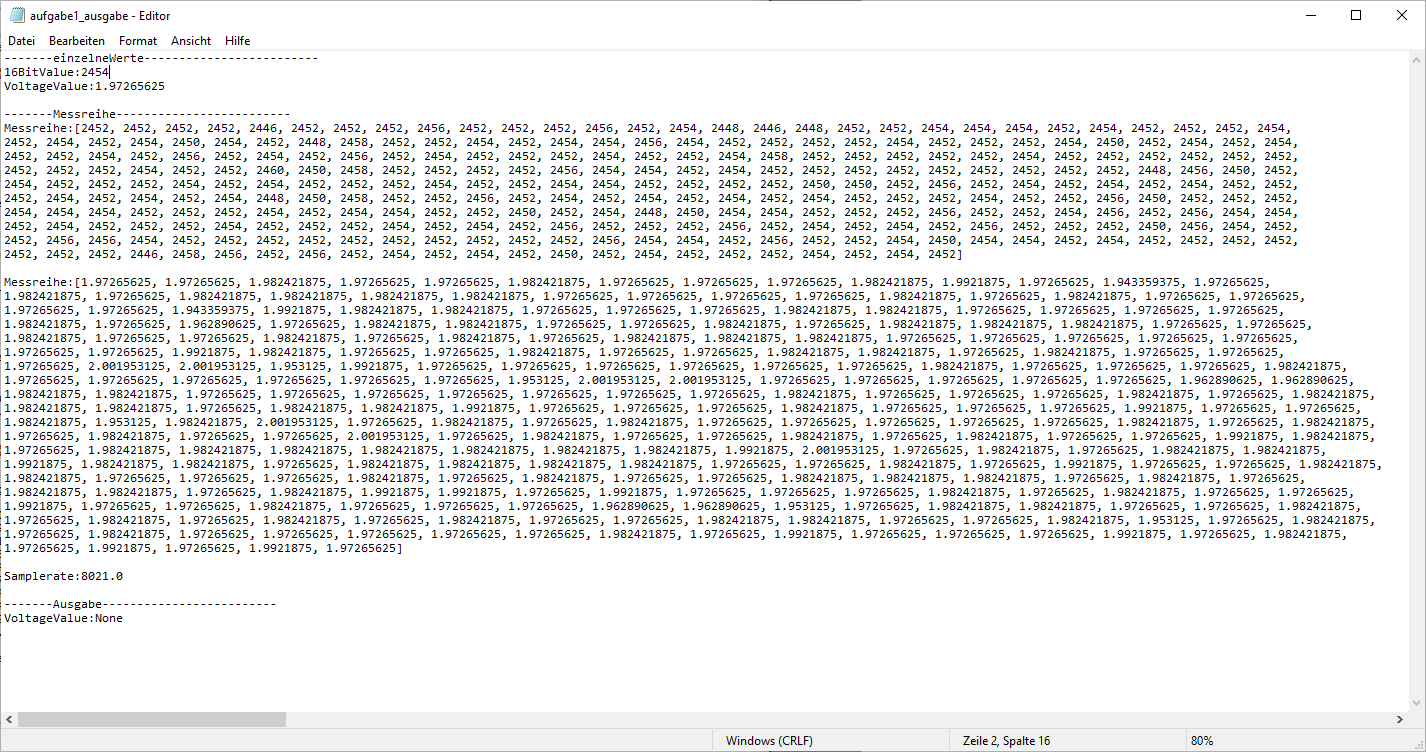
\includegraphics[width=\linewidth]{media/values}
	\caption{Konsolenausgabe als .txt Datei}
	\label{img:values}
\end{figure}
\section{Auswertung}
\label{chap:VERSUCH_1_AUSWERTUNG}
In dem zweiten Teil des ersten Versuches haben wir eine Konsoleneingabe auf die Karte ausgegeben. Dabei kann man Werte zwischen 0 und 5 Volt angeben.
\newline
Nachdem wir nun einen Wert von 3V in die Konsole durch das Pythonskript eingegeben haben, wurde von uns nun das Messgerät verwendet.
\newline
Im Anschluss haben wir eine Spannung von 3V mit dem Messgerät in dem Analogeingang gemessen.
\section{Interpretation}
\label{chap:VERSUCH_1_INTERPRETATION}
Unsere Karte hat die Konsoleneingabe akzeptiert, da der Wert am Ausgang der AD/DA Karte auch 3V betragen hat.
Somit ist die Karte und unser Skript funktionstüchtig.
\newline
\newline
Der Voltwert beträgt 1.97266V und die Samplerate beläuft sich auf 8021. Diese Samplerate ist auch die doppelte Nyquistfrequenz.
Der 16 Bitwert beträgt 2454.

%
% CHAPTER Versuch 2
%
\chapter{Versuch 2 - Genauigkeit der AD-Wandlung}
\label{chap:VERSUCH_2}

\section{Fragestellung, Messprinzip, Aufbau, Messmittel}
\label{chap:VERSUCH_2_FRAGESTELLUNG}
In diesem Versuch wird an der Spannungsquelle eine Spannung eingestellt, welche dann mit dem Mutlimeter Philips PM 2503, dem AD-Wandler und dem Feinmessgerät Keithley TRMS 179 (als Referenzwert) gemessen wird.
\begin{figure}[H]
	\centering\small
	\graphicspath{ {../versuch5/} }
	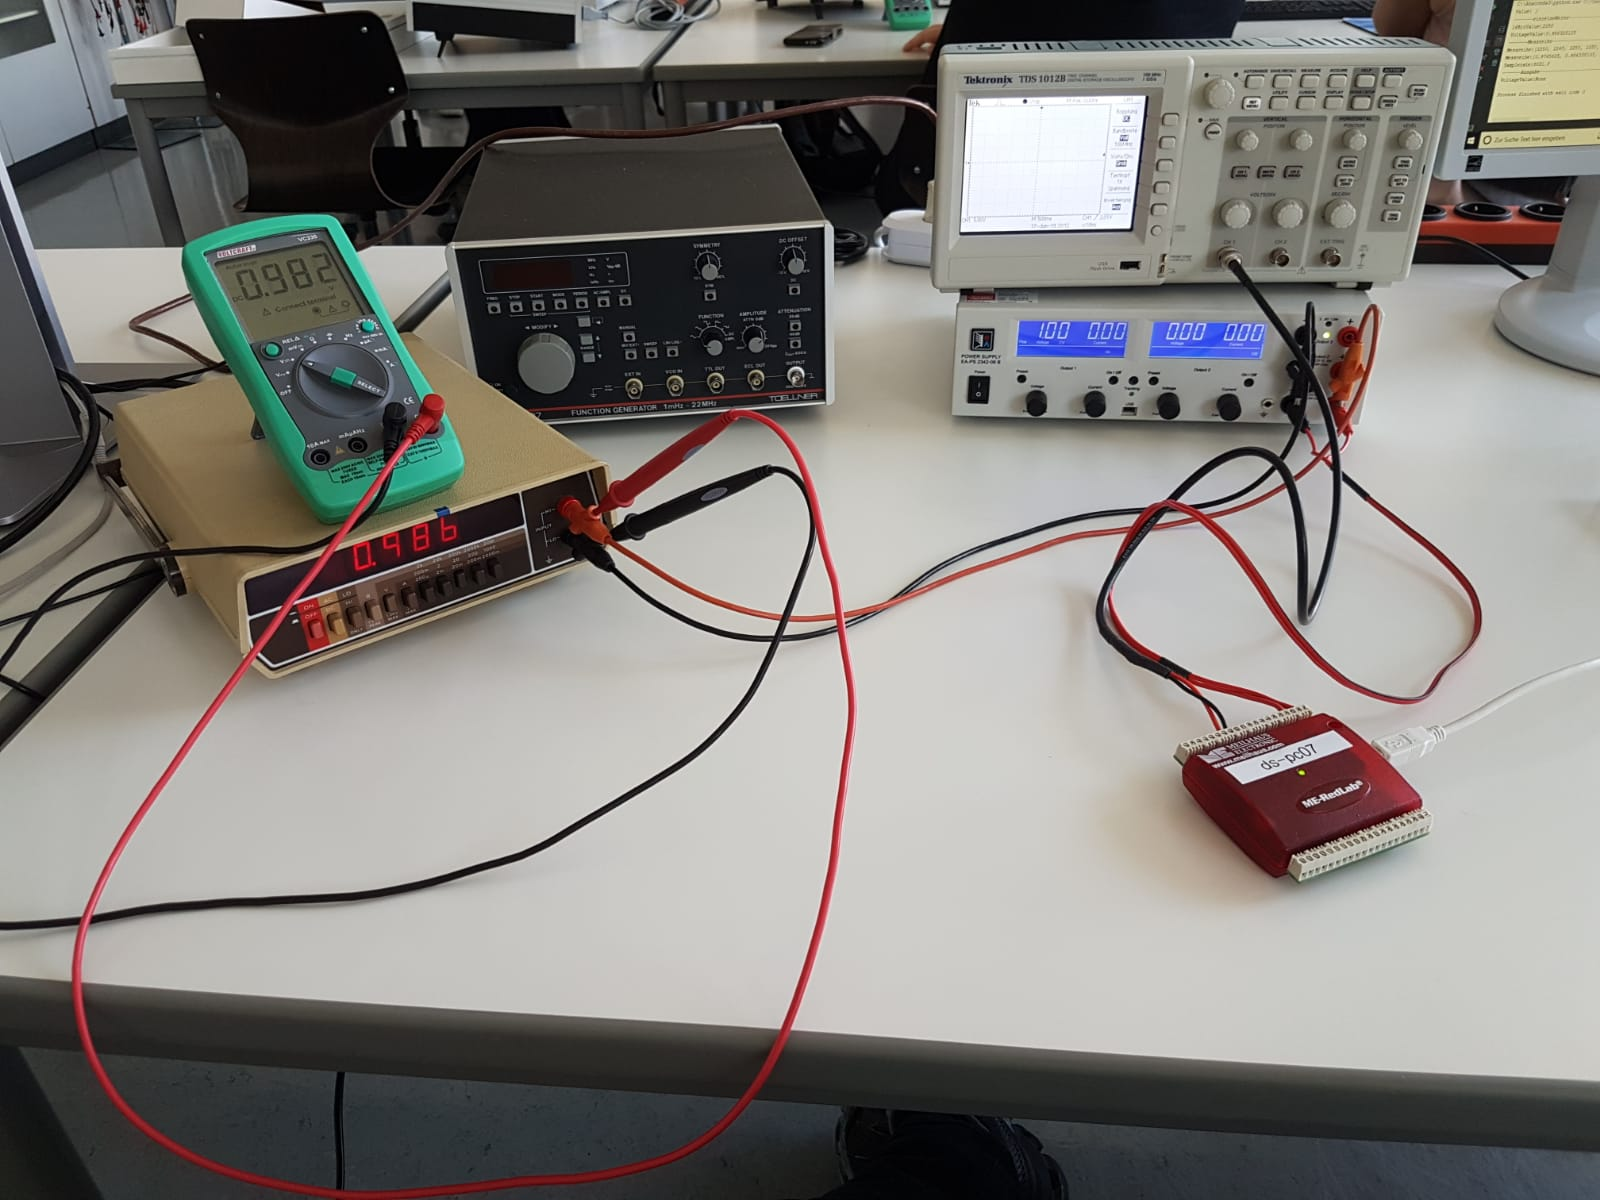
\includegraphics[width=.65\textwidth]{media/versuch2}
	\caption{Versuchsaufbau}
	\label{fig:V2}
\end{figure}

\section{Messwerte}
\label{chap:VERSUCH_2_MESSWERTE}
Folgende Messwerte wurden von uns während den Messungen zwischen 0 und 10 Volt notiert:
\begin{table}[H]
	\begin{tabular}{l|l|l|l|l|l}
		Spannung(V) & Feinmessgerät(V) & Multimeter & Messfehler & AD-Wandler & Messfehler\\
		\hline
		1 & 0.993 & 0.988 & 0.005 & 0.986 & 0.007\\
		2 & 2.049 & 2.04 & 0.009 & 2.041 & 0.008\\
		3 & 3.055 & 3.044 & 0.011 & 3.046 & 0.009\\ 
		4 & 4.065 & 4.05 & 0.015 & 4.052 & 0.013\\
		5 & 5.074 & 5.06 & 0.014 & 5.058 & 0.016\\
		6 & 5.987 & 5.96 & 0.027 & 5.976 & 0.011\\ 
		7 & 7.044 & 7.02 & 0.024 & 8.046 & 0.008\\
		8 & 8.054 & 8.03 & 0.024 & 8.046 & 0.008\\
		9 & 9.063 & 9.040 & 0.023 & 9.052 & 0.011\\
		10 & 10.073 & 10.04 & 0.033 & 9.961 & 0.012\\
	\end{tabular}
	\caption{Messwerte Feinmessgerät, Multimeter, AD-Wandler}
	\label{MWADWANDLER}
\end{table}

\section{Auswertung}
\label{chap:VERSUCH_2_AUSWERTUNG}
Der theoretische Quantisierungsfehler für den AD-Wandler beträgt
\begin{equation}
\Delta U\textsubscript{AD} = \frac{10V - 1V}{2\textsuperscript{11}} = 4.4mV
\end{equation}
Für das Multimeter ergibt sich aus den Messwerten die folgende Standardabweichung
\begin{equation}
S\textsubscript{M} = 9mV
\end{equation}
und für den AD-Wandler
\begin{equation}
S\textsubscript{AD} = 2.8mV
\end{equation}
\newpage
\section{Interpretation}
\label{chap:VERSUCH_2_INTERPRETATION}
Anhand der Standardabweichungen lässt sich feststellen, dass das Multimeter ungenauer ist, als der AD-Wandler. Die gemessene Standardabweichung von 2.8mV ist niedriger als der theoretische Quantisierungsfehler von 4.4mV. Daraus lässt sich schließen, dass die Messwerte im Fehlertoleranzbereichs des theoretischen Quantisierungsfehler liegen. Deshalb ist dieser theoretisch berechnete Wert für die AD-Wandlung plausibel.

%
% CHAPTER Versuch 3
%
\chapter{Versuch 3 - Genauigkeit der DA-Wandlung}
\label{chap:VERSUCH_3}

\section{Fragestellung, Messprinzip, Aufbau, Messmittel}
\label{chap:VERSUCH_3_FRAGESTELLUNG}
Hier sollen nun Analogwerte vom DA-Wandler gemessen werden.
Die DA-Wandler wird programmiert Spannungen auszugeben, die dann vom Oszilloskop gemessen werden.
Der Versuchsaufbau sieht dabei wie folgt aus:
\begin{figure}[H]
	\centering\small
	\graphicspath{ {../versuch5/} }
	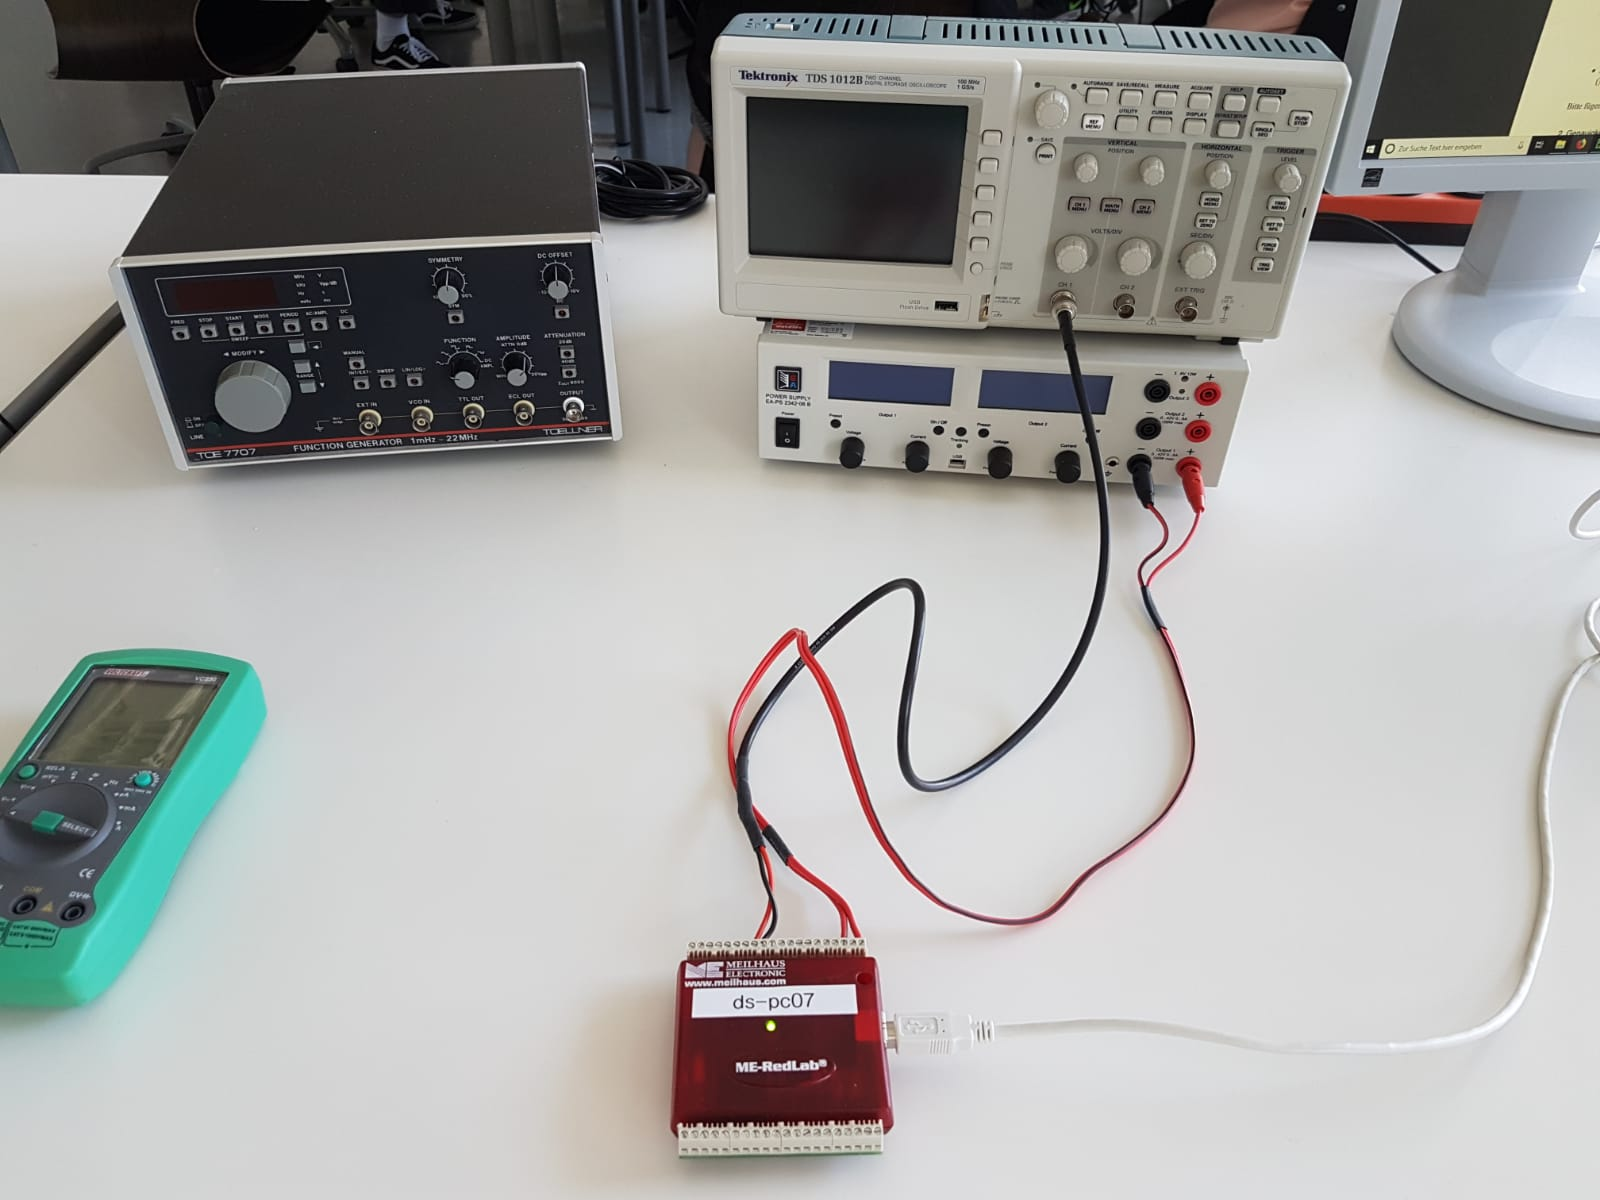
\includegraphics[width=.65\textwidth]{media/versuch3}
	\caption{Versuchsaufbau}
	\label{fig:V3}
\end{figure}
\section{Messwerte}
\label{chap:VERSUCH_3_MESSWERTE}
Folgende Messwerte wurden von uns bei den Messungen zwischen 0 und 5 Volt notiert:

\begin{table}[H]
	\centering
	\begin{tabular}{l|l|l}
		Spannung(V) & Oszilloskop(V) & Messfehler(V)\\
		\hline
		0.5 & 0.557 & 0.057\\
		1 & 1.05 & 0.05\\
		1.5 & 1.59 & 0.09\\
		2 & 2.08 & 0.08\\
		2.5 & 2.58 & 0.08\\
		3 & 3.11 & 0.11\\
		3.5 & 3.62 & 0.12\\
		4 & 4.15 & 0.15\\
		4.5 & 4.66 & 0.16\\
		5 & 5.14 & 0.14
	\end{tabular}
	\caption{Messwerte DA-Wandlung}
	\label{MWDAWANDLUNG}
\end{table}

\section{Auswertung}
\label{chap:VERSUCH_3_AUSWERTUNG}
Der theoretische Quantisierungsfehler für den DA-Wandler beträgt
\begin{equation}
\Delta U\textsubscript{DA} = \frac{5V - 0.5V}{2 \textsuperscript{10}} = 4.4mV
\end{equation}
Aus den Messwerten ergibt sich die folgende Standardabweichung
\begin{equation}
S\textsubscript{DA} = 38.5mV
\end{equation}

\section{Interpretation}
\label{chap:VERSUCH_3_INTERPRETATION}
Die Standardabweichung(38.5mV) liegt deutlich über dem theoretischen Quantisierungsfehler(4.4mV), was darauf schließen lässt, dass die Wandlung des digitalen Signals in ein analoges sehr fehlerbehaftet ist. Dazu tragen folgende Faktoren bei: thermisches Rauschen, Rundungsfehler, Überlastungsfehler.
%
% CHAPTER Versuch 4
%
\chapter{Versuch 4 - Zeitverhalten der DA-Wandlung}
\label{chap:VERSUCH_4}

\section{Fragestellung, Messprinzip, Aufbau, Messmittel}
\label{chap:VERSUCH_4_FRAGESTELLUNG}
Ziel des Versuchs ist zu sehen, wie genau sich mit einer Wandlerkarte eine Sinusschwingung erzeugen lässt.
Der Versuchversuchaufbau lautet folgendermaßen:
\newline
Der AD/DA Wandler wird via USB an den Computer angeschlossen.
Der AD/DA Wandler wird zudem an den Funktionsgenerator angeschlossen.
\newline
Der AD/DA Wandler wird zudem an das Oszilloskop an Channel1 angeschlossen.
\newline
Die Verbindung zum Oszilloskop wird verwendet um die Sinusschwinung auszugeben.
\newline
Das Python Programm (s. task4.py) errechnet ein Array von Sinuswerten mit 30 Werten pro Schwingung.
\begin{figure}[H]
	\centering\small
	\graphicspath{ {../versuch4/} }
	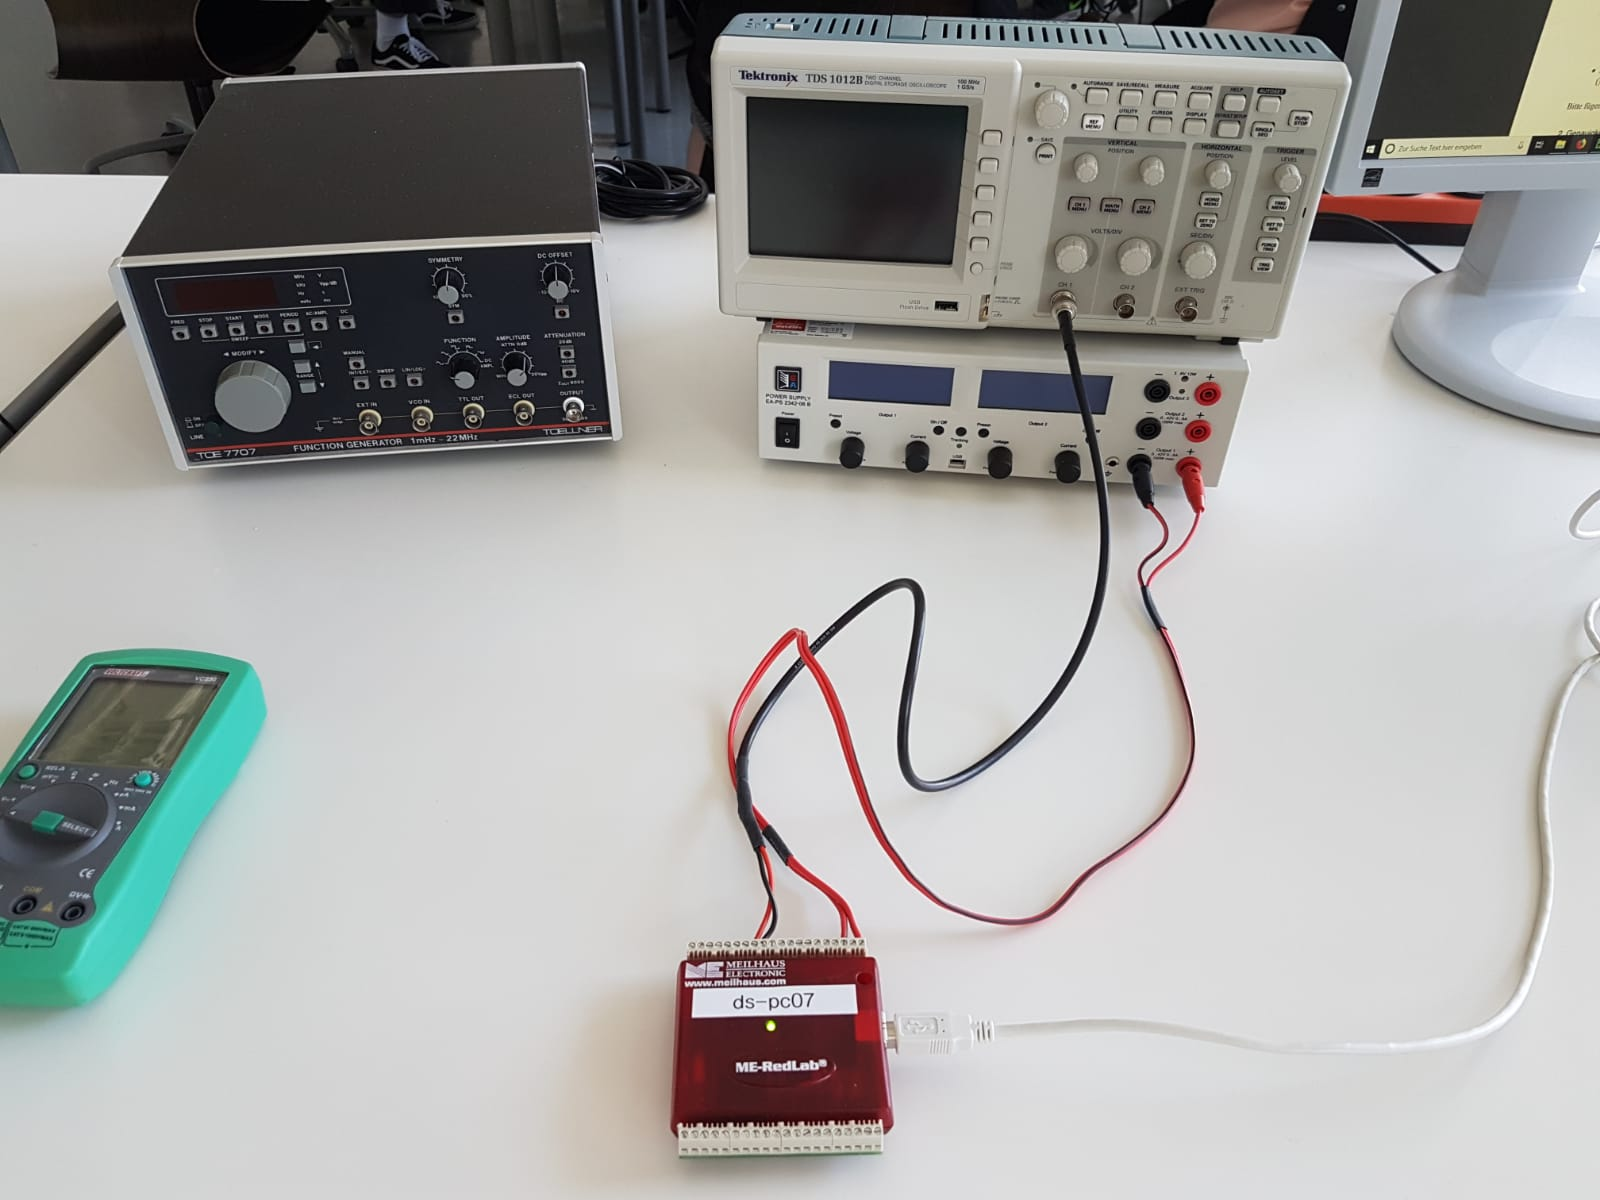
\includegraphics[width=.5\textwidth]{media/versuch3}
	\caption{Versuchsaufbau}
	\label{fig:TEIL1KOMPLETT}
\end{figure}
\newpage
\section{Messwerte}
\label{chap:VERSUCH_4_MESSWERTE}
Nachdem das Sinussignal von dem AD/DA Wandler zum Oszilloskopen geleitet wird, machen wir mit dem Programm auf dem Computer im Labor ein Screenshot des Oszilloskopen.
\newline
Das Ergebnis ist in dem folgenden Schaubild zu erkennen.
\begin{figure}[H]
	\centering\small
	\graphicspath{ {../versuch5/} }
	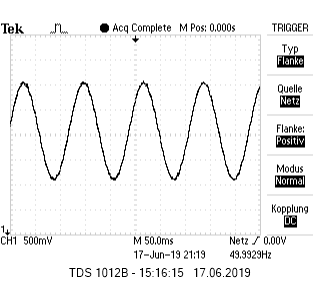
\includegraphics[width=.65\textwidth]{media/sinus}
	\caption{Ausgegebene Sinusspannung}
	\label{fig:TEIL1KOMPLETT}
\end{figure}

\section{Interpretation}
\label{chap:VERSUCH_4_INTERPRETATION}

Die Sinusspannung entspricht sehr gut einer realen Sinusschwingung, jedoch entsteht man aufgrund der kleinen Anzahl der Amplitudenstufen(30) ein Treppeneffekt, wodurch das Signal bei näherer Betrachtung leicht rauschig wirkt.

%
% CHAPTER Versuch 5
%
\chapter{Versuch 5 - Abtasttheorem}
\label{chap:VERSUCH_5}

\section{Fragestellung, Messprinzip, Aufbau, Messmittel}
\label{chap:VERSUCH_5_FRAGESTELLUNG}
Im fünften Versuch dürfen wir eine Abtastfrequenz zwischen 6000 und 8000 auswählen. Wir haben uns für eine Frequenz von 8000 entschieden. Mittels Python und dem RedLab-Befehl rl.cbInScanRate werden wir die tatsächliche Abtastfrequenz des AD-Wandlers für die Abtastfrequenz auslesen. 
\newline
Zudem haben wir die Nyquistfrequenz ermittelt.
Im Anschluss sollen wir von der halben Nyquistfrequenz bis zur doppelten Nyquistfrequenz, die Frequenz des Sinusgenerators variieren. 
Nach der Programmierung des Sinusgenerators, haben wir diese auf 7 verschiedene Frequenzen angewendet.
\newline
Im Anschluss daraufhin sollen die Kurven für das Protokoll plotten.
So bekommen wir im Anschluss für 7 verschiedene Frequenzen 7 verschiedene Plots.
\newline
In Abbildung ist es gut zu sehen, wie unser Aufbau erfolgt ist:
\newline
Der AD/DA Wandler wurde per USB an den Computer angeschlossen. Der AD/DA Wandler wurde ebenfalls auch noch an den Funktionsgenerator angeschlossen, welcher davor auf Sinusschwingungen eingestellt wurde.
\newpage
\section{Messwerte}
\label{chap:VERSUCH_5_MESSWERTE}
Die folgenden Messwerte sind entstanden, indem wir nun einen Sinuswert eingegeben haben in unseren Sinusgenerator, denn wir mittels Python programmiert haben.
Die Frequenz haben wir dabei auf 7 verschiedene Nyquistfrequenz eingestellt:
\begin{itemize}
\item 2000Hz
\item 3000Hz
\item 4010Hz
\item 5000Hz
\item 6000Hz
\item 7000Hz
\item 8020Hz
\end{itemize}

\begin{figure}[H]
   \begin{minipage}[b]{.5\linewidth} % [b] => Ausrichtung an \caption
      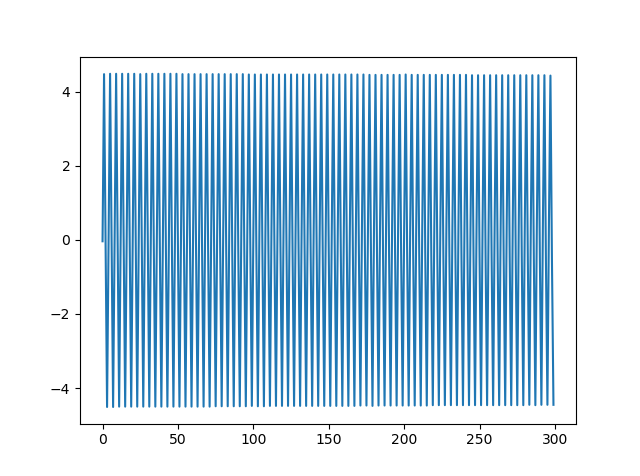
\includegraphics[width=\linewidth]{media/2000Hz}
      \caption{Messfrequenz von 2000Hz}
   \end{minipage}
   \begin{minipage}[b]{.5\linewidth} % [b] => Ausrichtung an \caption
      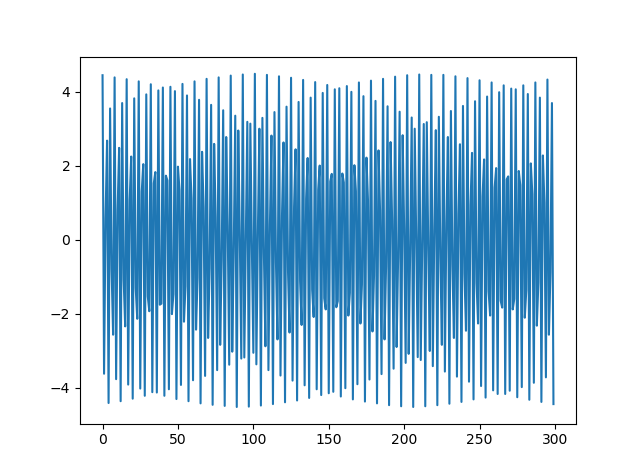
\includegraphics[width=\linewidth]{media/3000Hz}
      \caption{Messfrequenz von 3000Hz}
   \end{minipage}
\end{figure}

\begin{figure}[H]
   \begin{minipage}[b]{.5\linewidth} % [b] => Ausrichtung an \caption
      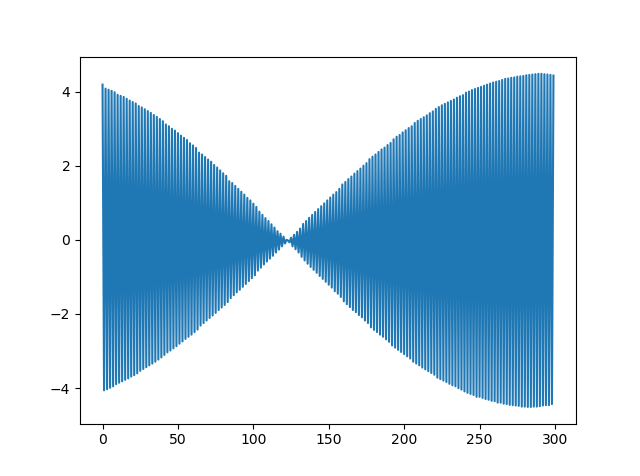
\includegraphics[width=\linewidth]{media/4010Hz}
      \caption{Messfrequenz von 4010Hz}
   \end{minipage}
   \begin{minipage}[b]{.5\linewidth} % [b] => Ausrichtung an \caption
      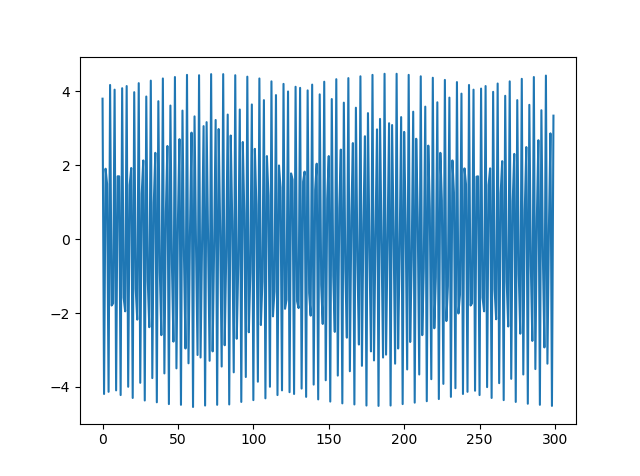
\includegraphics[width=\linewidth]{media/5000Hz}
      \caption{Messfrequenz von 5000Hz}
   \end{minipage}
\end{figure}

\begin{figure}[H]
   \begin{minipage}[b]{.5\linewidth} % [b] => Ausrichtung an \caption
      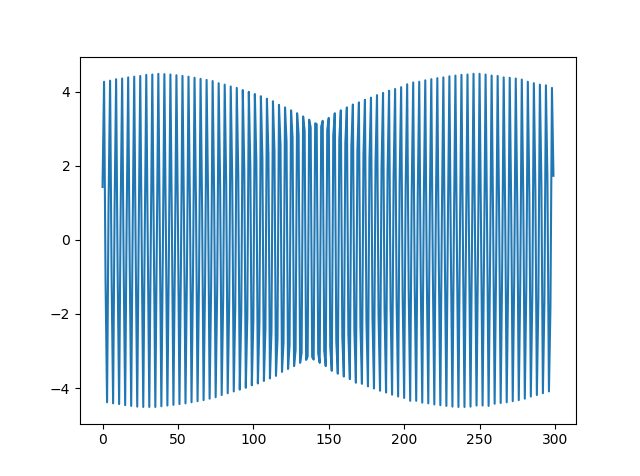
\includegraphics[width=\linewidth]{media/6000Hz}
      \caption{Messfrequenz von  6000Hz}
   \end{minipage}
   \begin{minipage}[b]{.5\linewidth} % [b] => Ausrichtung an \caption
      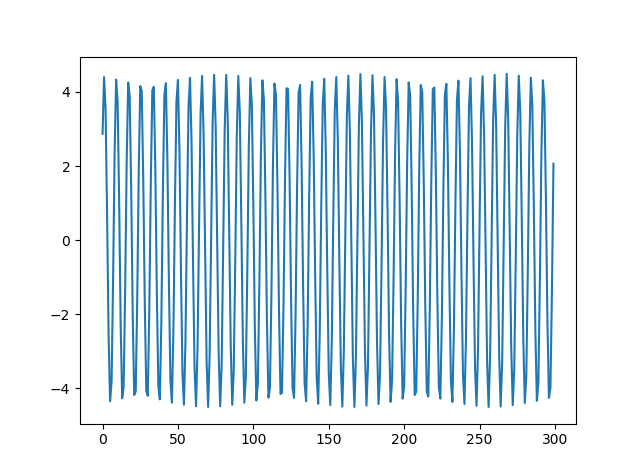
\includegraphics[width=\linewidth]{media/7000Hz}
      \caption{Messfrequenz von 7000Hz}
   \end{minipage}
\end{figure}

\begin{figure}[H]
   \begin{minipage}[b]{.5\linewidth} % [b] => Ausrichtung an \caption
      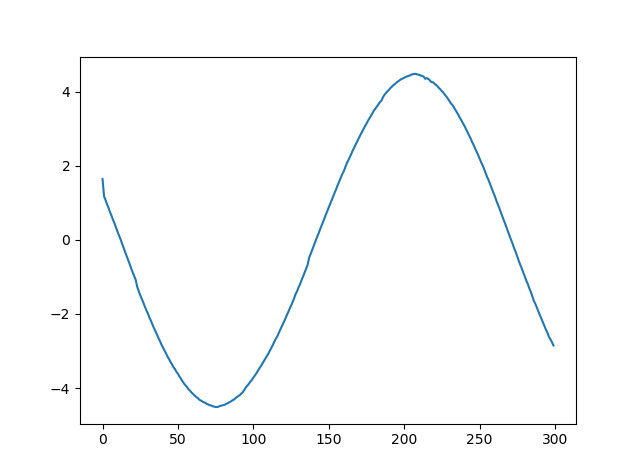
\includegraphics[width=\linewidth]{media/8020Hz}
      \caption{Messfrequenz von 8020Hz}
   \end{minipage}
\end{figure}

\newpage
\section{Auswertung}
\label{chap:VERSUCH_5_AUSWERTUNG}
Da wir von Anfang an eine Abtastfrequenz von 8000Hz verwendet haben, waren wir sehr nahe an der tatsächlichen Abtastfrequenz von 8021.
Diese haben wir durch den Befehl 
\newline
\textit{cbInScanRate(0, 0, 0, 8000)} erfahren. 
\newline
Da dies jedoch die doppelte Nyquistfrequenz ist, wollen wir noch die normale Nyquistfrequenz erfahren.
\newline
Dies wird logischerweise ermöglicht durch die Division der doppelten Nyquistfrequenz duch 2:
\newline
\newline
\textbf{8021 / 2 = 4010.5}
\newline
\newline

\section{Interpretation}
\label{chap:VERSUCH_5_INTERPRETATION}
In den Bildern 6.2, 6.3, 6.4 und 6.5 geschieht das sogenannte Aliasing.
\newline
Da die Abtastfrequenz bei diesen Plots kleiner ist als die doppelte Grundfrequenz, überlappen sich die Kopien des Spektrums.
\newline
Diese Überlappung wird Aliasing genannt.
\begin{figure}[hbt!]
	\centering
	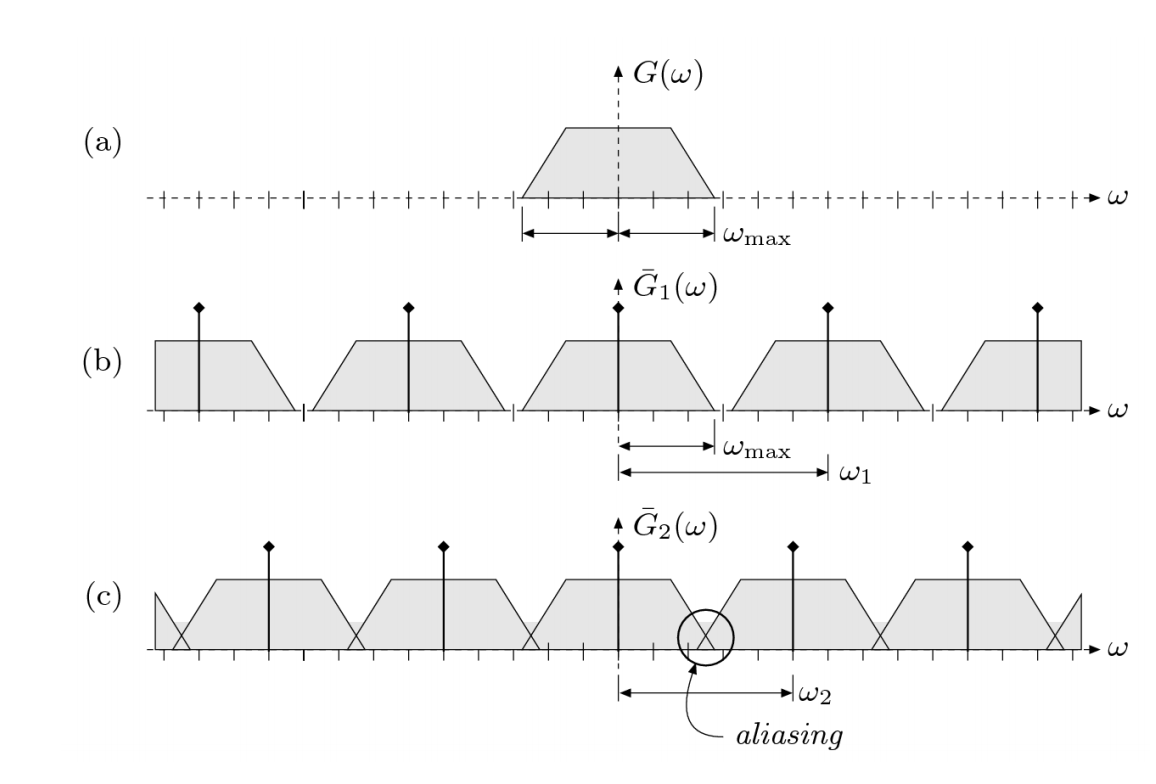
\includegraphics[width=.65\linewidth]{media/aliasing}
	\caption{Schaubild zu Aliasing}
	\label{img:Aliasing}
\end{figure}
\newpage
Bei den anderen Schaubildern 6.1, 6.6 und 6.7 geschieht kein Aliasing. 
\newline
Dafür muss die Abtastfrequenz größer sein, als die doppelte Grundfrequenz des Signals.
Bei der tatsächlichen Nyquistfrequenz von 4010.5Hz ist die Überlappung bezeihungsweise das Aliasing am größten.
\newline
Umso weiter sich die Abtastfrequenz von der Nyquistfrequenz entfernt, desto geringer wird das Aliasing.
\newline
Erst bei der Aufnahme der Nyquistfrequenz von 7000Hz, ist das Aliasing verschwunden.
Während der ersten Aufnahme noch kein Aliasing zu sehen, beginnt dies dafür dann bei der zweiten aufgenommenen Frequenz von 3000Hz.
Beim letzten Messwert von 8020Hz sieht man genau eine Schwingung, da sich die Frequenz nur um 1Hz von der doppelten Nyquistfrequenz(8021Hz) unterscheidet.

%
% CHAPTER Anhang
%
\renewcommand\thesection{A.\arabic{section}}
\renewcommand\thesubsection{\thesection.\arabic{subsection}}

\chapter*{Anhang}
\label{chap:APPENDIX}
\addcontentsline{toc}{chapter}{Anhang}
%\setcounter{chapter}{0}
\addtocounter{chapter}{1}
\setcounter{section}{0}

\section{Quellcode Aufgabe 1}
\label{chap:APPENDIX_SOURCECODE}

\lstinputlisting[
style=PYTHON,
frame=single,
caption=Versuch1.py,
captionpos=b,
firstnumber=45]{../versuch5/task1.py}
\newpage

\section{Quellcode Aufgabe 4}
\label{chap:APPENDIX_SOURCECODE}

\lstinputlisting[
style=PYTHON,
frame=single,
caption=Versuch4.py,
captionpos=b,
firstnumber=45]{../versuch5/task4.py}

\newpage

\section{Quellcode Aufgabe 5}
\label{chap:APPENDIX_SOURCECODE}

\lstinputlisting[
style=PYTHON,
frame=single,
caption=Versuch5.py,
captionpos=b,
firstnumber=45]{../versuch5/task5.py}

\section{Messprotokolle}
\label{chap:APPENDIX_SOURCECODE}

\begin{figure}[H]
	\centering\small
	\graphicspath{ {../versuch5/} }
	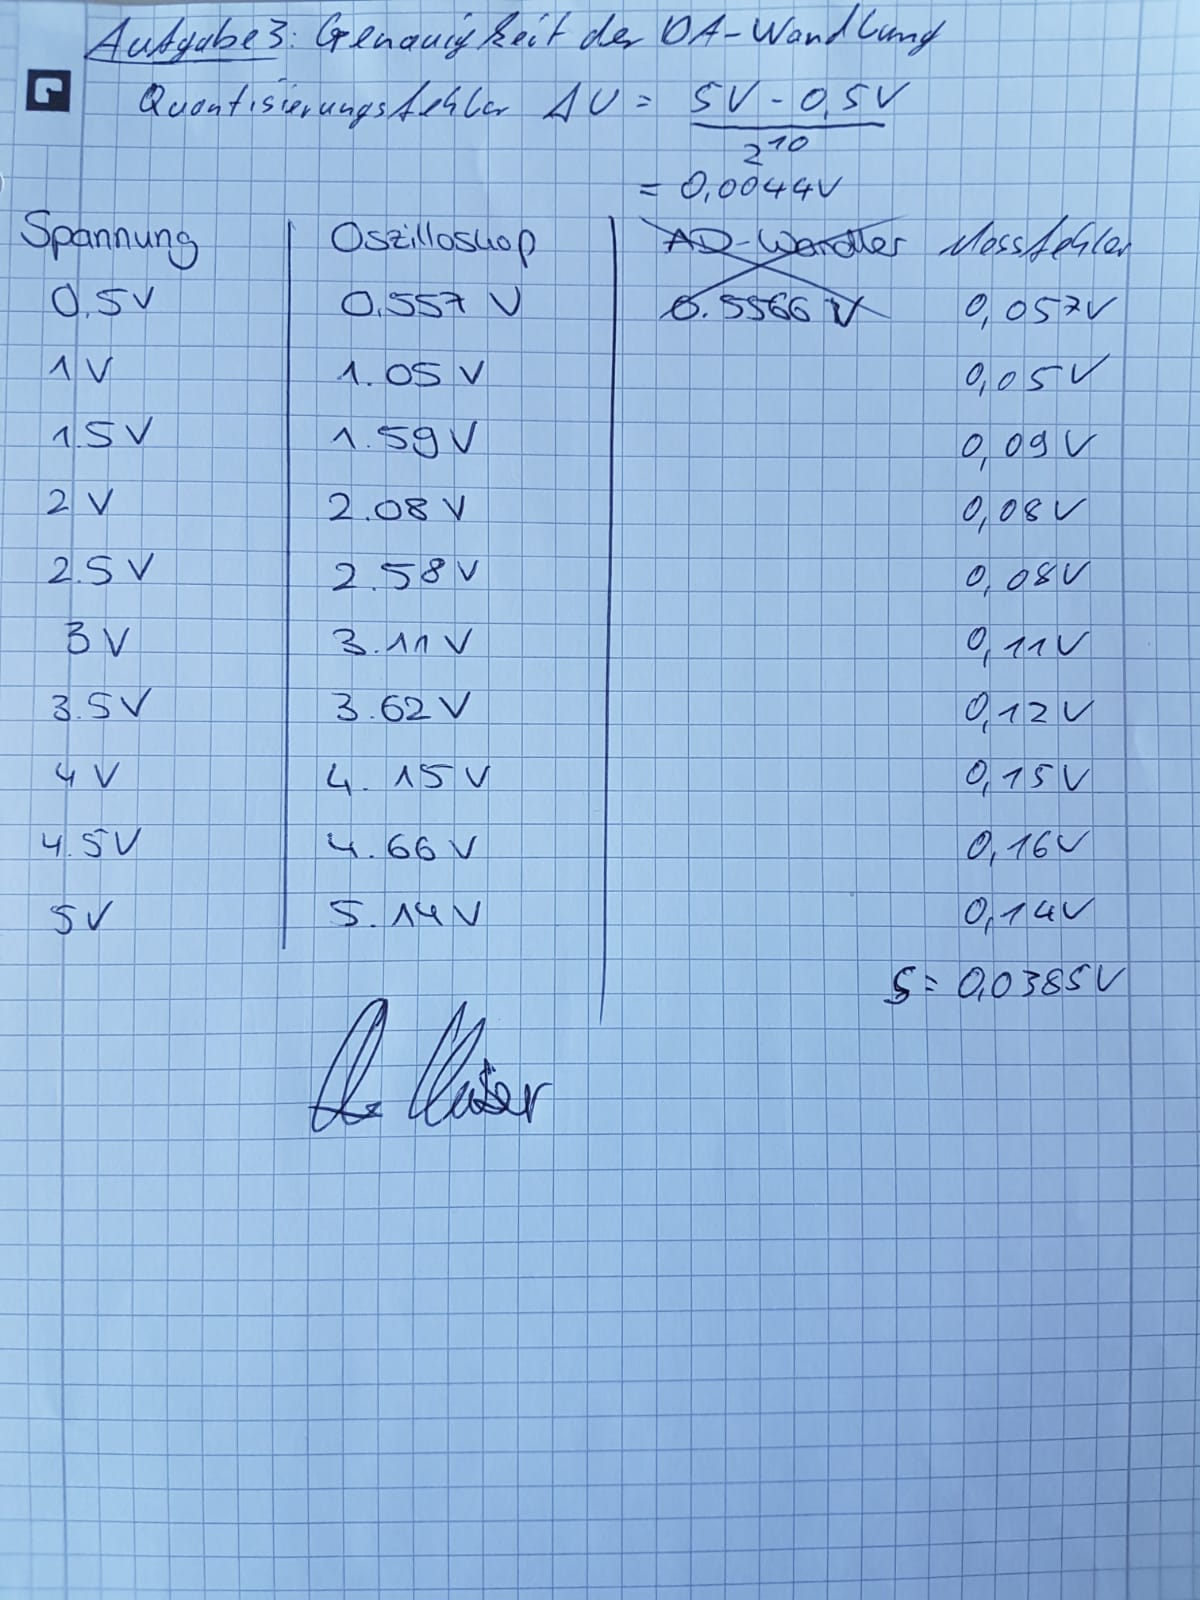
\includegraphics[width=.65\textwidth]{media/protokoll1}
	\caption{Protkoll Aufgabe 3}
	\label{fig:PROTOKOLL3}
\end{figure}

\begin{figure}[H]
	\centering\small
	\graphicspath{ {../versuch5/} }
	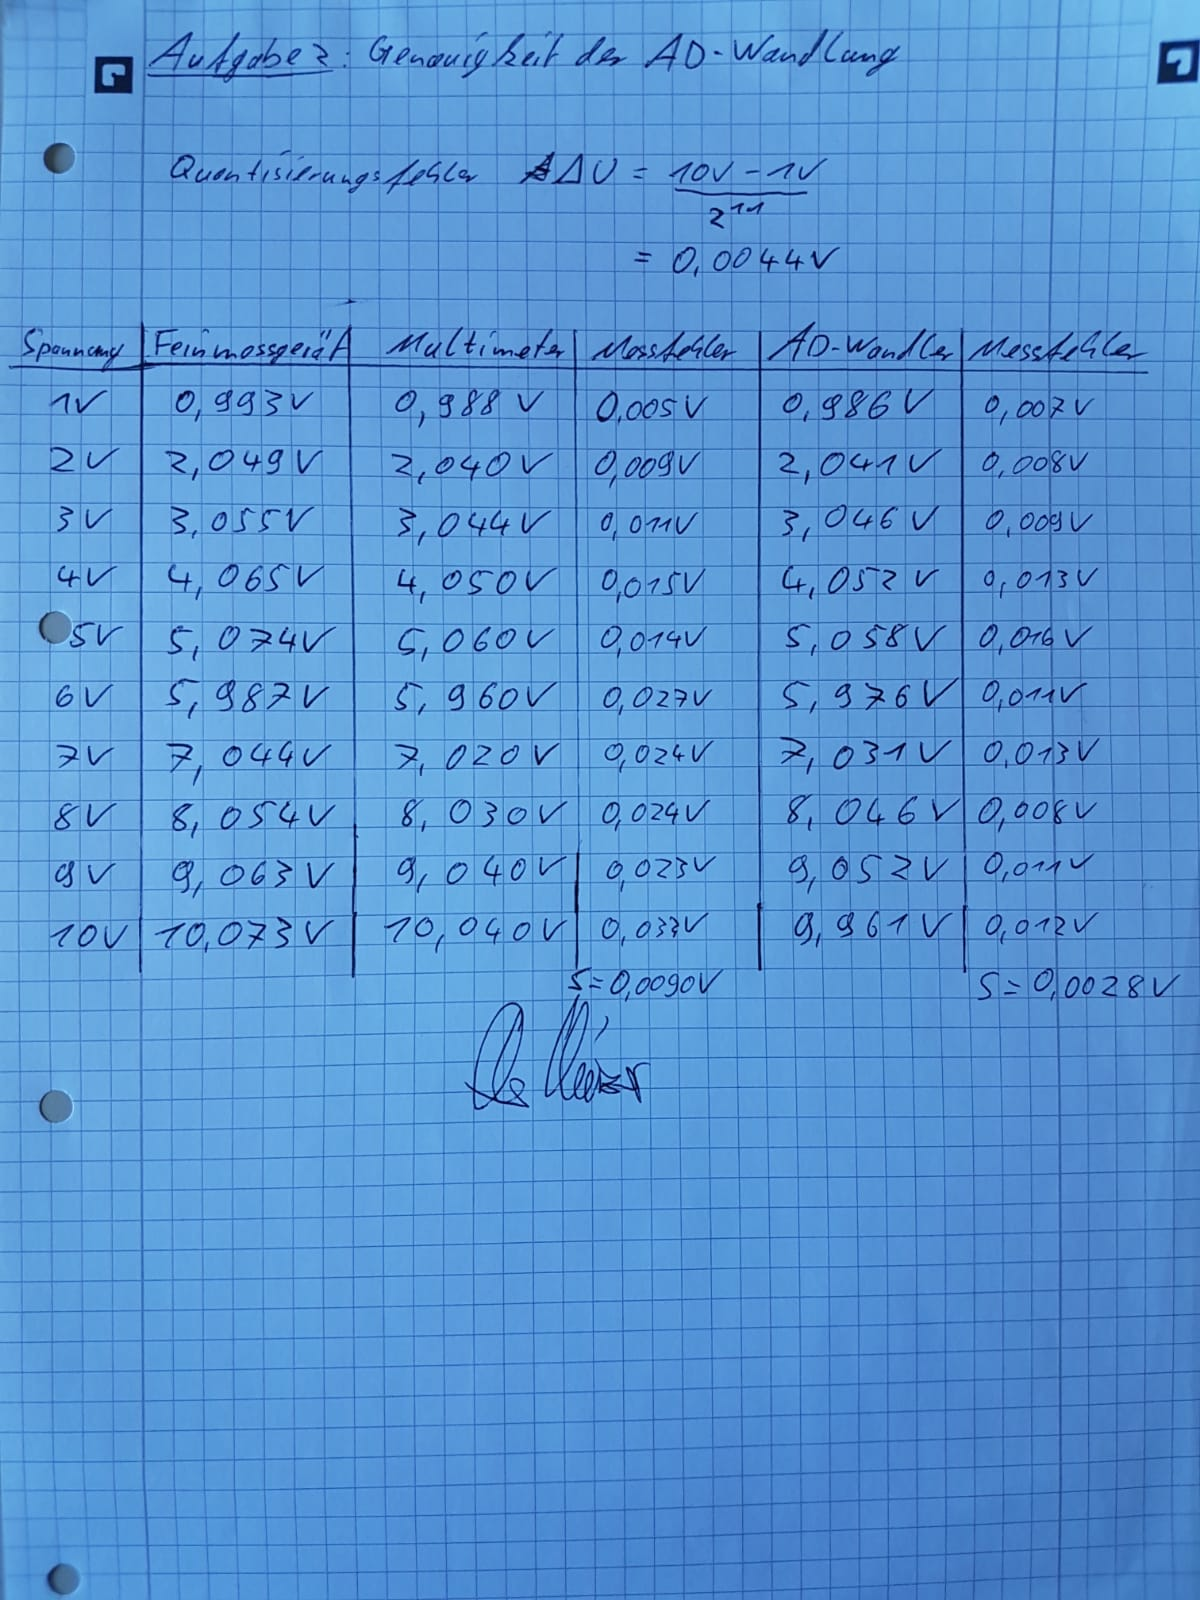
\includegraphics[width=.65\textwidth]{media/protokoll2}
	\caption{Protokoll Aufgabe 2}
	\label{fig:PROTOKOLL2}
\end{figure}

\end{document}
%------------------------------------
% ╔═╗╔╗╔╔╦╗  ╔╦╗╔═╗╔═╗╦ ╦╔╦╗╔═╗╔╗╔╔╦╗
% ║╣ ║║║ ║║   ║║║ ║║  ║ ║║║║║╣ ║║║ ║ 
% ╚═╝╝╚╝═╩╝  ═╩╝╚═╝╚═╝╚═╝╩ ╩╚═╝╝╚╝ ╩ 
%------------------------------------